% vi:ft=tex
\documentclass[utf8x,10pt,aspectratio=169]{beamer}
\usepackage{hyperref}

\mode<presentation>

\usetheme[pagenum,nosectionnum,heavyfont]{tud}
\usepackage[cache=false,outputdir=.texpadtmp]{minted}
\usepackage{graphics}

%\setbeameroption{show notes}
%\setbeamertemplate{note page}[plain]

\setbeamertemplate{footnote}
{
  \tiny
  \noindent%
  \insertfootnotemark~\insertfootnotetext
}

\titlegraphic{
	
\includegraphics[width=2cm]{img/cfaed.png}\hspace*{4.75cm}~%
	
\includegraphics[width=2cm]{img/cfaed.png}
}

\AtBeginSection[]
{
  \begin{frame}
    \frametitle{Table of Contents}
    \tableofcontents[currentsection]
  \end{frame}
}

\title{Extending and completing Ÿauhau}
\author{Justus Adam, supervised by Sebastian Ertel and Andres Goens}
\date{\today}
\datecity{Dresden}

 \def\insertframetitle{} 
\begin{document}

\normalsize
\maketitle

\begin{frame}[fragile]{Motivation}
	
\begin{minted}{Clojure}
(defn common-friends [x y]
  (intersection (friends-of x) (friends-of y)))

(defn friends-of [x]
  (fetch (FriendsOf. x)))
\end{minted}
\pause
\begin{itemize}[<+->]
	\item Batching, Caching and Concurrency desired
	\item Retaining concise and straight forward code
\end{itemize}

\end{frame}
\addtocounter{framenumber}{-1}
\begin{frame}[fragile]
	\frametitle{Motivation}

\begingroup
\definecolor{green(html/cssgreen)}{rgb}{0.0, 0.5, 0.0}
\catcode`\@=\active
\def@#1@{\textcolor{green(html/cssgreen)}{#1}}
\begin{minted}[escapeinside=||]{Clojure}
(|@defalgo@| common-friends [x y]
  (intersection (friends-of x) (friends-of y)))

(|@defalgo@| friends-of [x]
  (fetch (mk-req (FriendsOf. x) data-source)))
\end{minted}
\endgroup
\begin{itemize}
	\item Batching, Caching and Concurrency desired
	\item Retaining concise and straight forward code
	\item Ÿauhau solves issue with minimal difference in code
\end{itemize}

\end{frame}

\begin{frame}{Goals}
	\pause
	\begin{block}{Current status}
		\begin{itemize}[<+->]
			\item Ÿauhau supports a base transformation on a dataflow graph
			\item The structure of the graph does not reflect control flow
		\end{itemize}
	\end{block}
	\pause
	\begin{block}{Tasks}
		\begin{itemize}[<+->]
			\item Handling control flow
			\item Iteration/mapping with \texttt{smap}
			\item Conditional execution with \texttt{if}
			\item Semantics of side effects (writes)
		\end{itemize}
	\end{block}
\end{frame}

\begin{frame}{Table of Contents}	
	\tableofcontents
\end{frame}

\section{Application}

\begin{frame}{Application}
	\begin{itemize}
		\item Large scale, distributed systems (Facebook, Amazon, Twitter)
		\item Haskell library Haxl\footnote{Simon Marlow, Louis Brandy, Jonathan Coens, and Jon Purdy. 2014. There is no fork: an abstraction for efficient, concurrent, and concise data access. ICFP '14.}
		\item Clojure library Muse\footnote{Alexey Kachayev. 2015. Reinventing Haxl: Efficient, Concurrent and Concise Data Access. https://www.youtube.com/watch?v=T-oekV8Pwv8}
		\item Scala implementation Stitch by Twitter\footnote{Jake Donham. 2014. Introducing Stitch. https://www.youtube.com/watch?v=VVpmMfT8aYw} (closed source)
		\item Ÿauhau as an Ohua plugin\footnote{Sebastian Ertel, Andrés Goens, Justus Adam and Jeronimo Castrillon. Ÿauhau: Concise Code and Efficient I/O Straight from Dataflow. POPL '17. In submission.}
	\end{itemize}
\end{frame}

\section{Ÿauhau Overview}

\begin{frame}{Ohua}
	\begin{itemize}[<+->]
		\item Ÿauhau hooks into the Ohua\footnote{Sebastian Ertel, Christof Fetzer, and Pascal Felber. 2015. Ohua: Implicit Dataflow Programming for Concurrent Systems. PPPJ '15} compiler
		\item Parallelisation framework based on dataflow\footnote{Arvind and David E. Culler. 1986. Dataflow architectures. In Annual review of computer science vol. 1}\footnote{J. B. Dennis. 1974. First version of a data flow procedure language. In Programming Symposium, Proceedings Colloque sur la Programmation}
		\item Stateful functions and algorithms (\texttt{defalgo}) as abstraction
	\end{itemize}
\end{frame}

\begin{frame}[fragile]{Base transformation}
	
	\begin{columns}[T]
		\column{.4\textwidth}
		\begin{itemize}
			\item<2-> Rewrites high level algorithms
		\end{itemize}	
		\column{.6\textwidth}

\begingroup
\definecolor{green(html/cssgreen)}{rgb}{0.0, 0.5, 0.0}
\catcode`\@=\active
\def@#1@{\textcolor{green(html/cssgreen)}{#1}}
\begin{minted}[escapeinside=||]{Clojure}
(|@defalgo@| common-friends [x y]
  (intersection 
    (friends-of x) 
    (friends-of y)))

(|@defalgo@| friends-of [x]
  (fetch (mk-req (FriendsOf. x) 
                 data-source)))
\end{minted}
\endgroup
	\end{columns}
	
\end{frame}

\addtocounter{framenumber}{-1}

\begin{frame}[fragile]{Ÿauhau base transformation}
	
	\begin{columns}[T]
		\column{.4\textwidth}
		\begin{itemize}
			\item Rewrites high level algorithms
			\item Operates on dataflow ir
		\end{itemize}	
		\column{.6\textwidth}
		\begin{minted}{Clojure}
(let [[x y] (algo-in)
      a (mk-req (FriendsOf. x) data-source)
      b (mk-req (FriendsOf. y) data-source)
      c (fetch a)
      d (fetch b)
      e (intersection a b)]
  e)
		\end{minted}
	\end{columns}
	
\end{frame}

\addtocounter{framenumber}{-1}

\begin{frame}[fragile]{Ÿauhau base transformation}
	
	\begin{columns}[T]
		\column{.4\textwidth}
		\begin{itemize}
			\item Rewrites high level algorithms
			\item Operates on dataflow ir
			\item Traverses dataflow graph along dependencies
			\item<2-> Collect fetches, replace with accumulator
			\item<3-> Transformation is very simple and naive
		\end{itemize}	
		\column{.6\textwidth}
		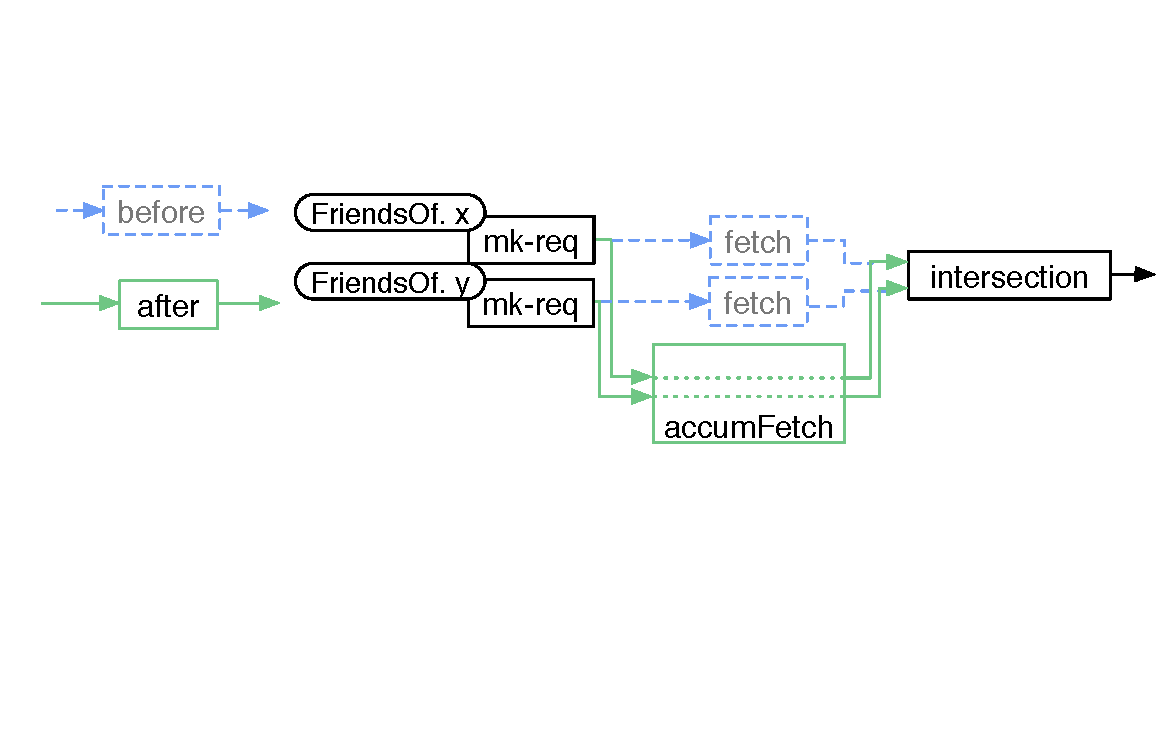
\includegraphics[width=\textwidth]{graphs/yauhau-transformation}
	\end{columns}
	
\end{frame}

\section{\texttt{smap} rewrite}
\begin{frame}{\texttt{smap} rewrite}
	\begin{columns}
		\column{0.4\textwidth}	
		\begin{itemize}
			\item Split inner graph around fetch
		\end{itemize}
		\column{0.6\textwidth}
		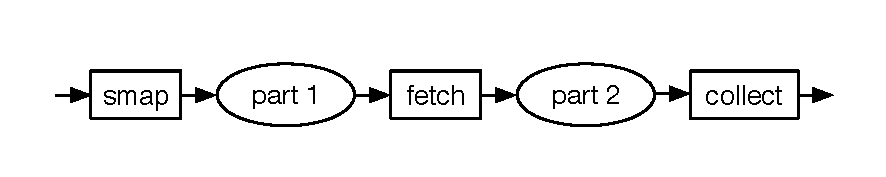
\includegraphics[width=\textwidth]{graphs/smap-rewrite-original}
	\end{columns}
		
\end{frame}

\addtocounter{framenumber}{-1}

\begin{frame}{\texttt{smap} rewrite}
	\begin{columns}
		\column{0.4\textwidth}	

		\begin{itemize}
			\item Split inner graph around fetch
			\item insert \texttt{collect} and \texttt{smap} around fetch
			\item<2-> Build tree of requests
		\end{itemize}
		\column{0.6\textwidth}
		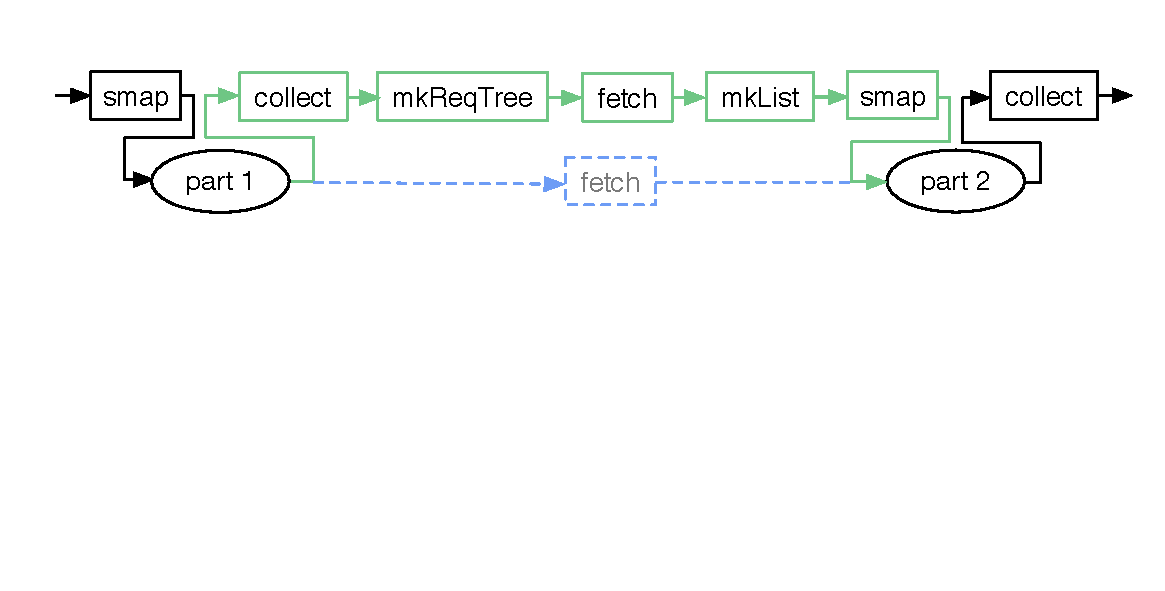
\includegraphics[width=\textwidth]{graphs/smap-rewrite}
	\end{columns}
		
\end{frame}

\section{\texttt{if} rewrite}

\begin{frame}{\texttt{if} rewrite}
	\begin{columns}
		\column{0.4\textwidth}
		\begin{itemize}[<+->]
			\item Split inner graph around fetch
		\end{itemize}
		\column{0.6\textwidth}
		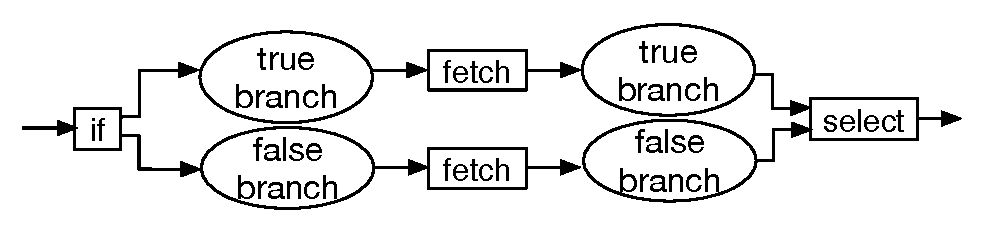
\includegraphics[width=\textwidth]{graphs/basic-if-rewrite-original}
	\end{columns}
\end{frame}

\begin{frame}{\texttt{if} rewrite}
	\begin{columns}
		\column{0.4\textwidth}
		\begin{itemize}
			\item Split inner graph around fetch
			\item Replace two fetches with one being selectively given the active request
			\item<2-> Push result to the continuation of the active branch using the initial condition
		\end{itemize}
		\column{0.6\textwidth}
		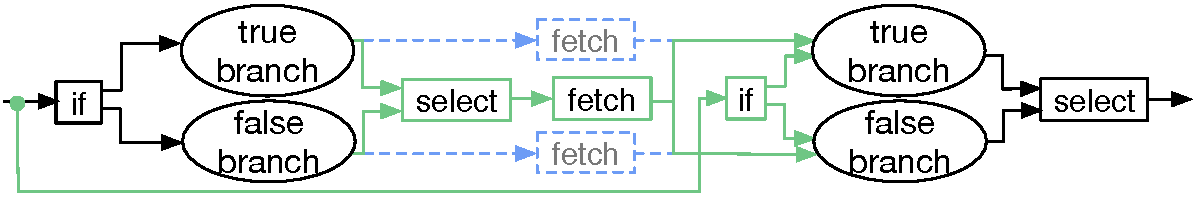
\includegraphics[width=\textwidth]{graphs/basic-if-rewrite}
	\end{columns}
\end{frame}

\addtocounter{framenumber}{-1}

\begin{frame}{\texttt{if} rewrite}
	\begin{columns}
		\column{0.4\textwidth}
		\begin{itemize}[<+->]
			\item Problem if unequal number of fetches on branches
			\item Solution: Insert extra fetches
		\end{itemize}
		\column{0.6\textwidth}
		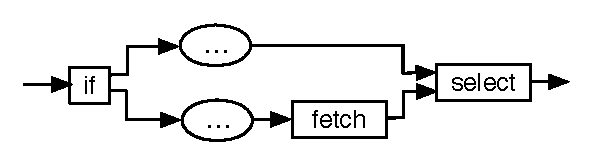
\includegraphics[width=\textwidth]{graphs/insert-empty-fetches}
	\end{columns}
\end{frame}
%
\addtocounter{framenumber}{-1}

\begin{frame}{\texttt{if} rewrite}
	\begin{columns}
		\column{0.4\textwidth}
		\begin{itemize}
			\item Problem if unequal number of fetches on branches
			\item Solution: Insert extra fetches
			\item Use NoOp (empty) requests
		\end{itemize}
		\column{0.6\textwidth}
		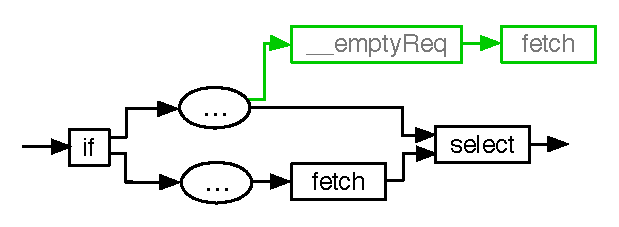
\includegraphics[width=\textwidth]{graphs/insert-empty-fetches-inserted}
	\end{columns}
\end{frame}
\section{Generalising to Context}
\begin{frame}{Generalising to Context}
	\begin{itemize}[<+->]
		\item Handle arbitrary graphs with conditionals, maps etc
		\item These structures are often interleaved
		\item Ease handling of complex nested stacks
	\end{itemize}
\end{frame}

\begin{frame}{Context}
	
	\begin{columns}
		
		\column{0.4\textwidth}
		\begin{itemize}[<+->]
		
			\item Hidden graph structures unified into context
			\item Context is property of subgraphs emerging from node labels
			\item Has a marker for begin and end
			\item Inherited property
			\item Subcontexts are always fully enclosed
			
		\end{itemize}
		
		\column{0.6\textwidth}
		
		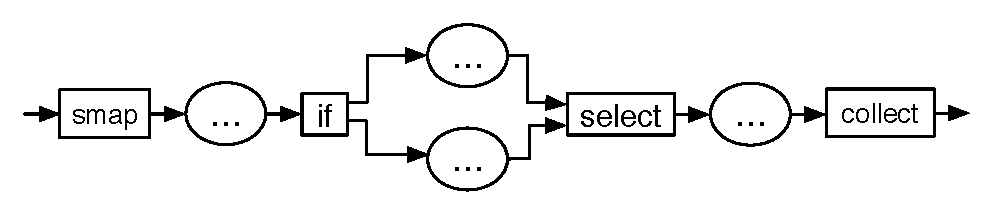
\includegraphics[width=\textwidth]{graphs/context-example}
			
	\end{columns}


	
\end{frame}

\begin{frame}{Finding context}

	\begin{columns}
		\column{0.4\textwidth}
	
		\begin{itemize}[<+->]
			\item Context recognition is done at compile time
			\item If a context opening node is found annotate subgraph
			\item Resolve full context stack by following the parent context references
		\end{itemize}
	
		\column{0.6\textwidth}
		
		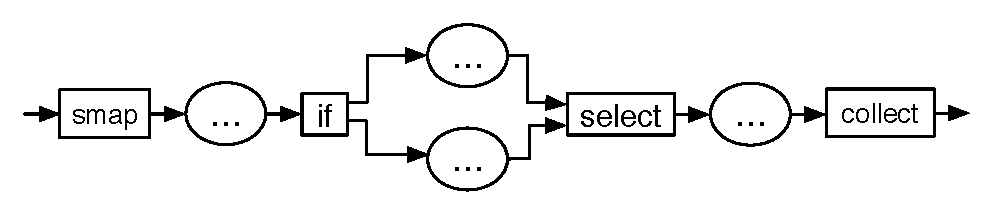
\includegraphics[width=\textwidth]{graphs/context-example}
	\end{columns}
	
\end{frame}

\begin{frame}{Finding context}

	\begin{columns}
		\column{0.4\textwidth}
	
		\begin{itemize}
			\item Context recognition is done at compile time
			\item If a context opening node is found annotate subgraph
			\item Resolve full context stack by following the parent context references
			\item<2-> Hinges on the ``fully enclosing'' property
		\end{itemize}
	
		\column{0.6\textwidth}
		
		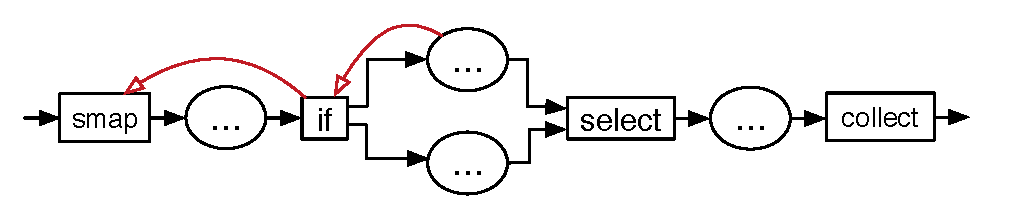
\includegraphics[width=\textwidth]{graphs/context-resolution-example}
	\end{columns}
	
\end{frame}

\begin{frame}{Handling arbitrary graphs}
	
	\begin{itemize}
		\item Calculate contexts for each fetch
		\item Contexts are unwound in order of descending nesting level
		\item Unwinding is interleaved
	\end{itemize}
\end{frame}
\section{Side Effect Semantics}
\begin{frame}[fragile]{Side Effects in Algorithms}
	\begin{columns}
		\column{0.4\textwidth}
		\begin{itemize}
			\item Execution order depends entirely on data dependencies
		\end{itemize}
		\column{0.6\textwidth}
		\begingroup
\definecolor{green(html/cssgreen)}{rgb}{0.0, 0.5, 0.0}
\catcode`\@=\active
\def@#1@{\textcolor{green(html/cssgreen)}{#1}}
\begin{minted}[escapeinside=||]{Clojure}
(|@defalgo@| main []
  (let [write-result 
        (write (WriteReq. "my-data") 
               data-source)
        fetch-data 
        (fetch (mk-req (Payload. "constant") 
               data-source))]
    (compute fetch-data write-result)))
		\end{minted}
		\endgroup
		
	\end{columns}
\end{frame}

\begin{frame}{Side Effects in Algorithms}
	\begin{columns}
		\column{0.4\textwidth}
		\begin{itemize}
			\item Execution order depends entirely on data dependencies
		\end{itemize}
		\column{0.6\textwidth}
		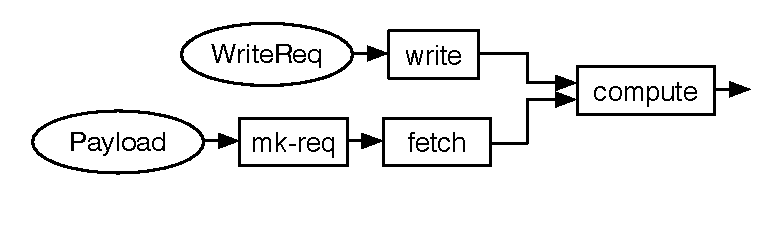
\includegraphics[width=\textwidth]{graphs/write-semantics-base}
		
	\end{columns}
\end{frame}

\begin{frame}[fragile]{Seq}
	\begin{columns}
		\column{0.4\textwidth}
		\begin{itemize}
			\item Execution order depends entirely on data dependencies
			\item Can be enforced using \texttt{seq} operator
		\end{itemize}
		\column{0.6\textwidth}
		\begingroup
\definecolor{green(html/cssgreen)}{rgb}{0.0, 0.5, 0.0}
\catcode`\@=\active
\def@#1@{\textcolor{green(html/cssgreen)}{#1}}
\begin{minted}[escapeinside=||]{Clojure}
(|@defalgo@| main []
  (let [write-result 
        (write (WriteReq. "my-data") 
               data-source)
        enforced 
        (seq write-result 
             (fetch (mk-req 
                      (Payload. "constant") 
                      data-source)))]
    (compute enforced write-result)))
		\end{minted}
		\endgroup
		
	\end{columns}
\end{frame}

\begin{frame}[fragile]{Side Effects across Algorithms}
	\begin{columns}
		\column{0.4\textwidth}
		
		\begin{itemize}
			\item Execution order depends entirely on data dependencies
			\item Can be enforced using \texttt{seq} operator
			\item Should be implicit from data dependencies
		\end{itemize}
		
		\column{0.6\textwidth}
		\begingroup
\definecolor{green(html/cssgreen)}{rgb}{0.0, 0.5, 0.0}
\catcode`\@=\active
\def@#1@{\textcolor{green(html/cssgreen)}{#1}}
\begin{minted}[escapeinside=||]{Clojure}
(|@defalgo@| does-read [x]
  (compute 
    (fetch (mk-req (Payload. "constant") 
                   data-source)) 
    x))
(|@defalgo@| does-write []
  (write (WriteReq. "my-data") data-source)
  ...)
(|@defalgo@| main []
  (does-read (does-write))
		\end{minted}
		\endgroup
		
	\end{columns}
\end{frame}

\begin{frame}{Enforcing Execution Order}

	\begin{itemize}[<+->]
		\item Exploring and evaluating different approaches
		\item Combining expected semantics and efficiency
	\end{itemize}
	
	\pause
	
	\begin{block}{Current approach}
		\begin{itemize}
			\item \texttt{seq}`ing fetches to algorithm boundary
			\item for `unconnected' fetches following writes
			\item Vice versa for `unconnected' writes following reads
		\end{itemize}
	\end{block}
	\pause
	\begin{block}{Open questions}
		\begin{itemize}
			\item Always enabled?
			\item Scope?
		\end{itemize}
	\end{block}

\end{frame}

\section{Experiments and Evaluation}

\begin{frame}{Experiments and Evaluation}
	Verifying correctness (program semantics) and performance in comparison to Haxl and Muse for:
	
	\pause
	
	\begin{enumerate}
		\item Modularised graphs (functions/algorithms)
		\item Graphs with map operations (\texttt{smap})
		\item Graphs with conditionals (\texttt{if})
	\end{enumerate}
	
	\pause
	
	This requires extensions to our random code generator to allow generation of correct code with
	
	\pause
	
	\begin{enumerate}
		\item Randomly generated functions
		\item Map operations using randomly generated functions
		\item Conditionals, with and without forcibly prefetched branches
	\end{enumerate}
	
\end{frame}

\begin{frame}
	The end. Thank you for listening. \\ \\
	Slides are available at \href{http://static.justus.science/presentations/extending-yauhau.pdf}{http://static.justus.science/presentations/extending-yauhau.pdf}
\end{frame}

\appendix

\begin{frame}[fragile]{Haxl Implementation details}

	\begin{columns}
	
		\column{0.4\textwidth}
		\begin{itemize}
			\item Applicative functors denote independent data fetches
			\item Monad bind retrieved data
			\item Requests are GADT's encoding result type
		\end{itemize}
		\column{0.6\textwidth}
		\begin{minted}{Haskell}
commonFriends :: Id -> Id -> GenHaxl [Id]
commonFriends x y = 
    intersection <$> friendsOf x 
                 <*> friendsOf y

friendsOf :: Id -> GenHaxl [Id]
friendsOf = dataFetch . FriendsOf
		\end{minted}		
	\end{columns}
	
\end{frame}

\begin{frame}[fragile]{Muse implementation detail}
	\begin{columns}
		\column{0.4\textwidth}
		\begin{itemize}
			\item Similar syntax to Haxl
			\item fmap/\texttt{<\$>} (\texttt{<\$>} and \texttt{<*>}), flat-map (\texttt{>>=})
			\item Uses free monad to build an AST
			\item Traverses AST to find fetch rounds
		\end{itemize}
		\column{0.6\textwidth}
		\begin{minted}{Clojure}
(defn common-friends [x y]
  (<$> intersection 
    (friends-of x) 
    (friends-of y)))

(defn friends-of [x]
  (FriendsOf. x))
  
(defrecord FriendsOf [id]
  MuseAST
  (...))
		\end{minted}
	\end{columns}

\end{frame}

\begin{frame}{Graphs}
	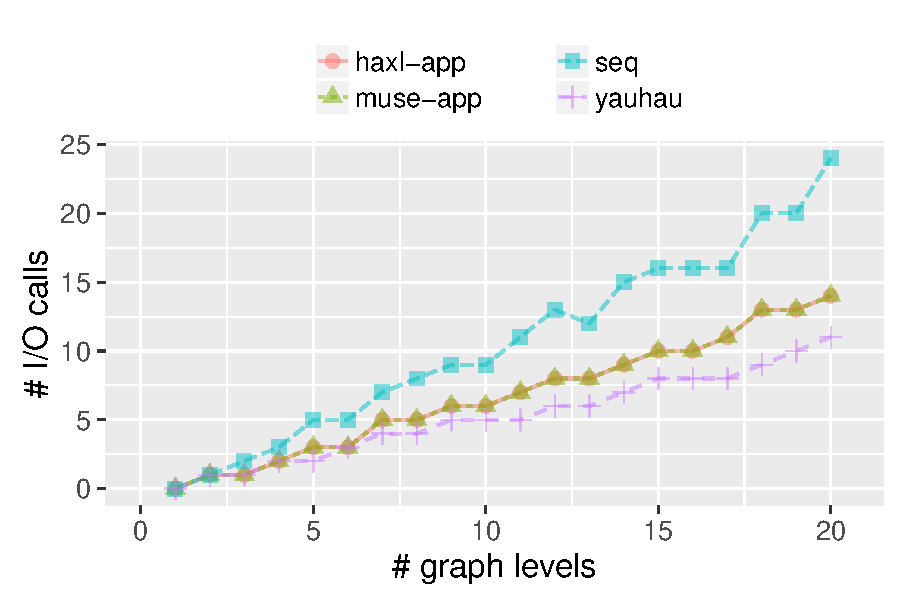
\includegraphics[width=0.5\textwidth]{plots/baseline}
	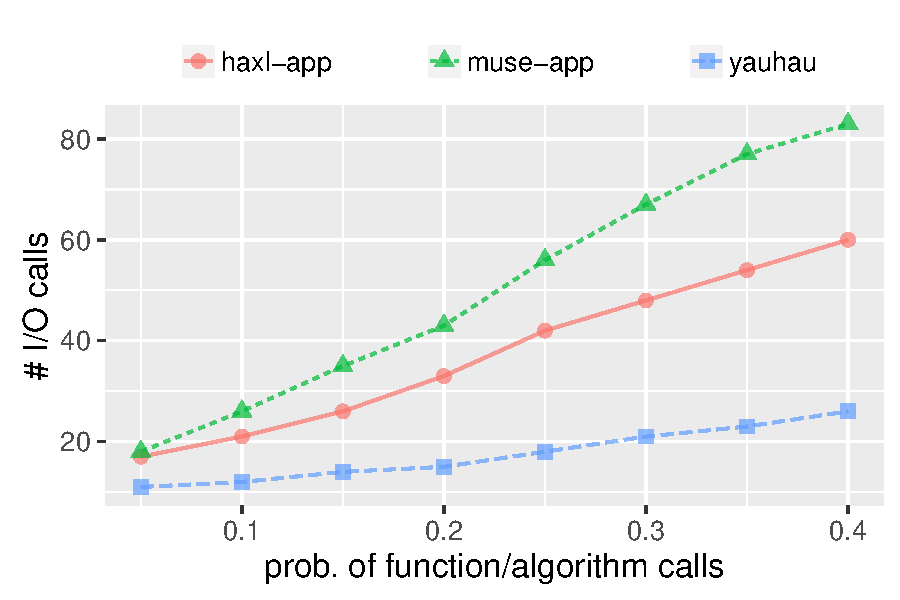
\includegraphics[width=0.5\textwidth]{plots/functions}
	
	Left: Baseline comparison. Right: Performance with functions.

\end{frame}

\begin{frame}{Graphs}
	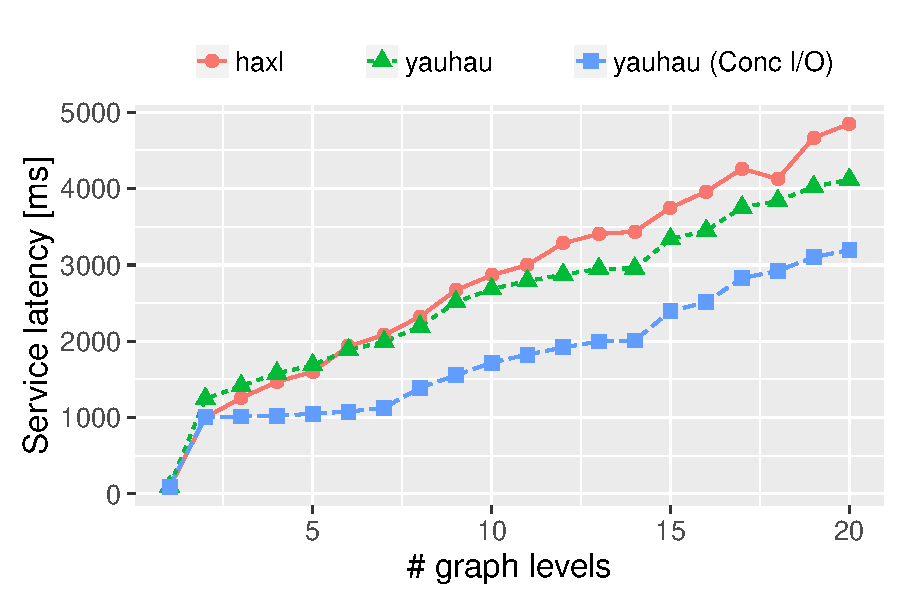
\includegraphics[width=0.5\textwidth]{plots/io-imbalance}
	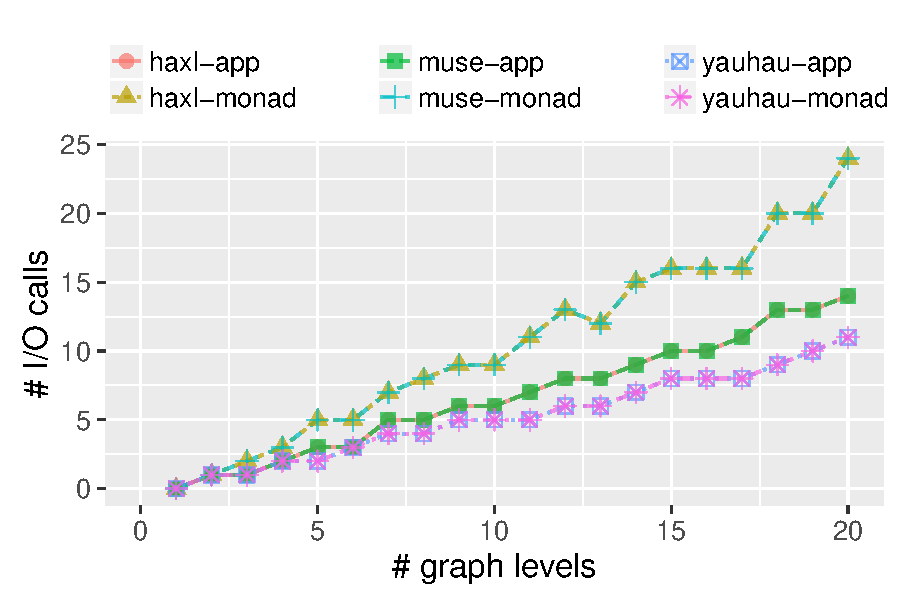
\includegraphics[width=0.5\textwidth]{plots/monad-vs-applicative}
	
	Left: Mixed latency data sources. Right: Performance across code styles.
\end{frame}

\begin{frame}[fragile]{Base transformation -- Details}
	\begin{columns}
		\column{0.4\textwidth}
		\begin{itemize}
			\item Simulates program execution
			\item Maintains set of created data (bindings)
			\item At each step `call' all non-fetch functions with satisfied inputs
			\item If no further function can be called dispatch round
		\end{itemize}
		\column{0.6\textwidth}
		\begin{minted}{Clojure}
(let [[x y] (algo-in)
      a (mk-req (FriendsOf. x) data-source)
      b (mk-req (FriendsOf. y) data-source)
      c (fetch a)
      d (fetch b)
      e (intersection a b)
  e)
		\end{minted}
	\end{columns}

\end{frame}

\end{document}

























